\section{Introduction\label{introduction}}

This paper shows an application of reinforcement learning for congestion reduction by mixed-autonomy, where both automated and human-driven vehicles present on traffic\cite{Wu:EECS-2018-132}. Some studies demonstrate that even a small number of vehicles in congested traffic can reduce huge amount of fuel consumption\cite{Wu:EECS-2018-132}.\\
Since 28\% of energy consumption in the U.S. is due to the transportation\cite{U.S.EnergyInformationAdministration2017}, and congestion can increase the fuel consumption\cite{Treiber2008}, reducing traffic congestion saves large amount of energy. 
To control the system-level traffic velocity, both model-based and model-free methods have been studied so far. The model-based methods give analytical solutions to maximize the traffic efficiency, but the situation it can be utilized is very limited. For example, the model-based controllers "Follower Stopper" and "PI with Saturation" \cite{Stern2018} can reduce the congestion in a ring road, but it doesn't give the optimal solution in the complex environments such as bottleneck and figure-eight(see Fig.\ref{fig:envs}). Due to the complex model of the real world traffic, the model-based methods may not work in many situations. 

On the other hand, model-free reinforcement learning(RL) has a potential to solve complex problems. For example, \cite{Mnih2013} trains an agents which solves Atari games at superhuman levels, and \cite{Silver2017} demonstrates that a RL agent outperforms a human Go player. \cite{Vinitsky2018} applies some state-of-the-art RL algorithms to complex traffic shown in Fig. \ref{fig:envs}, and most of the methods achieve better score than the situation with only human driven car. 

This research extends that previous work\cite{Kreidieh2018} and develops more practical agent using multi-agents method. A remaining problem in \cite{Kreidieh2018} is that it only uses one agent to control multiple cars. It's not flexible when the number of the car changes. Moreover, from the view of cyber security, one master node controlling the acceleration of multiple cars is dangerous. To train the agents, a policy gradient algorithm, Proximal Policy Optimization(PPO)\cite{Schulman2017} is used. The traffic simulator used in this work is Flow\cite{Wu2017}. It contains some benchmarks of practical traffic situations shown as \ref{fig:envs}, and it is easy to apply reinforcement learning agents to Flow. 

Finally, this paper shows the performance of imitation learning for the traffic control task. Generally, it is difficult to design a reward function for reinforcement learning. One of the solutions for reward design problem is to learn from an expert agent using imitation learning. To apply imitation learning, Generative Adversarial Imitation Learning(GAIL)\cite{Ho} is used in this research.

\begin{figure}[]
    \begin{center}
    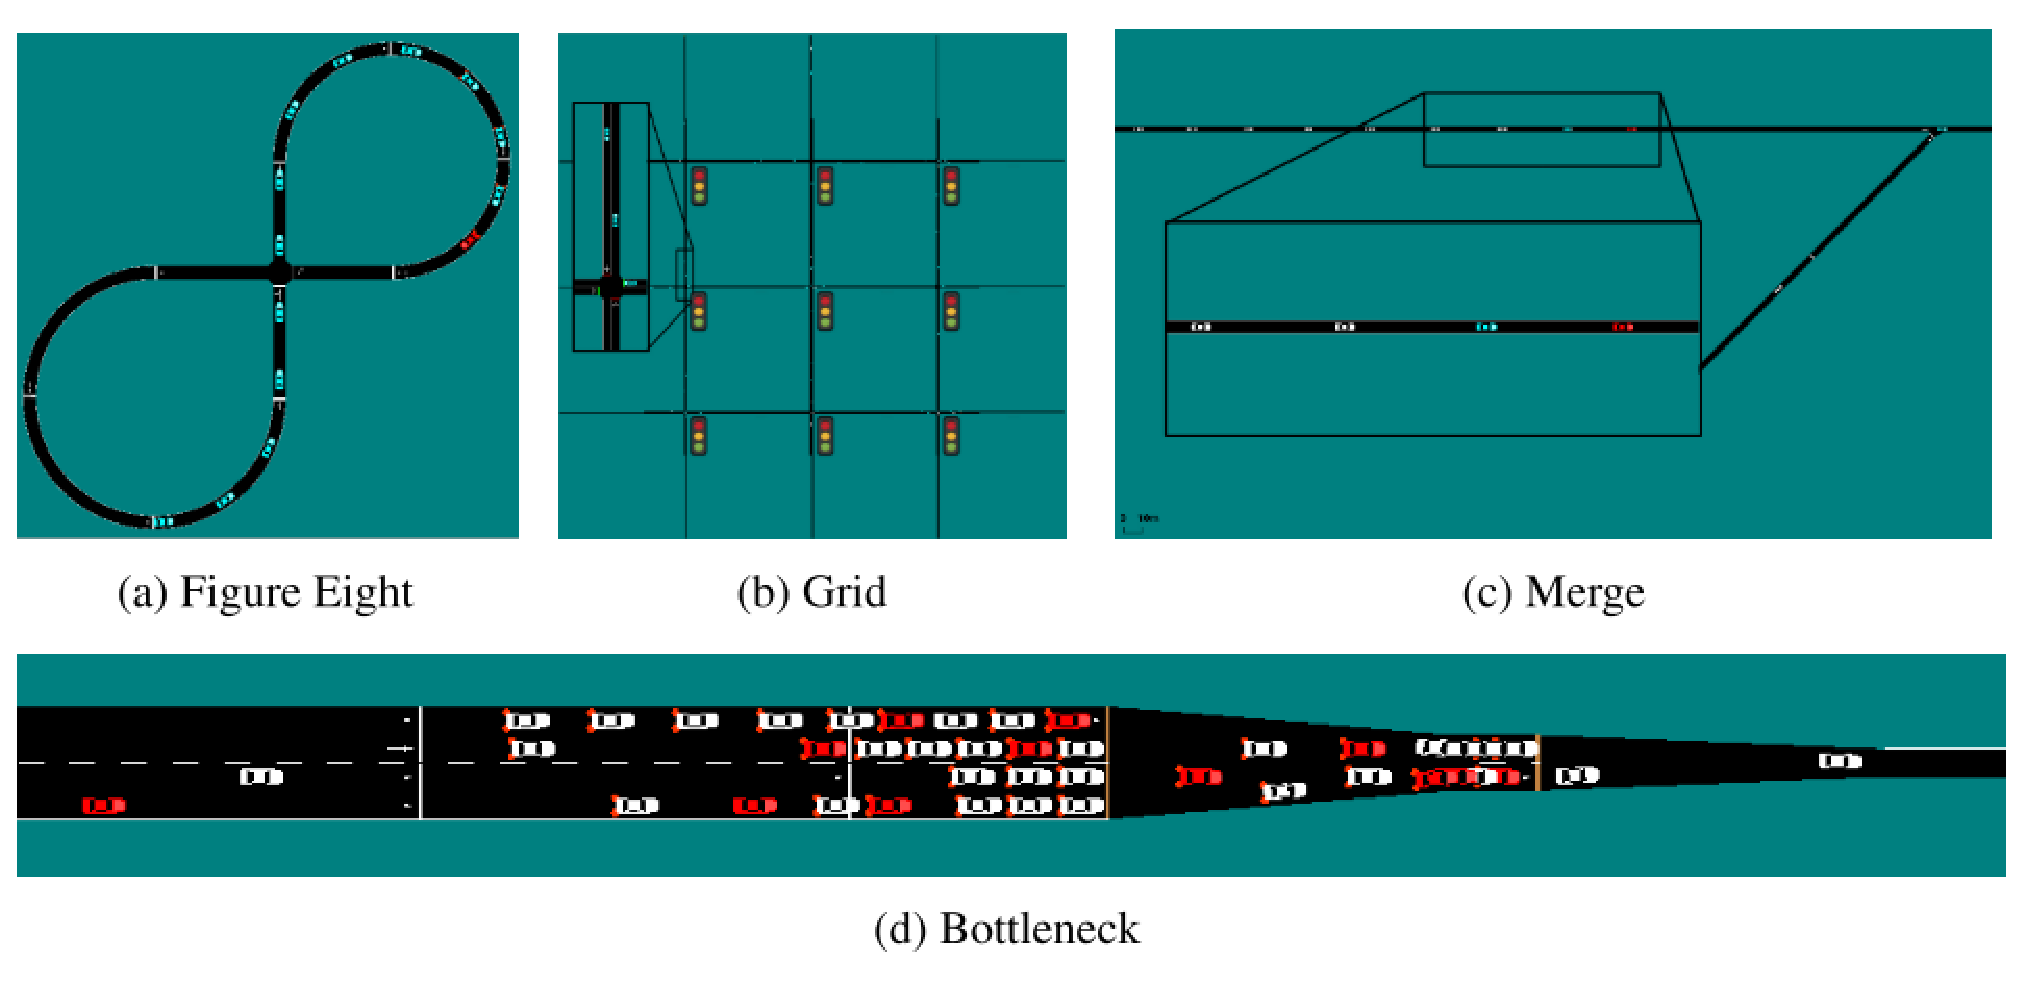
\includegraphics[width=9cm]{img/envs.eps}
    \caption{Complex traffic environments in "flow" (cited from \cite{Vinitsky2018})}
    \label{fig:envs}
    \end{center}
\end{figure}
%ここに画像が入る また、FLOWの結果を出して強化学習のほうが最適解を出せることを示す。